\setcounter{chapter}{0}

\chapter{Изучение работы шины AXI}

В данном разделе приведены диаграммы, иллюстрирующие процесс рукопожатия и пакетного чтения.

\section{Симуляция программы общего варианта}
Каналы позволяют сформировать конвейерные транзакции чтения и записи. Последовательность событий транзакции чтения можно представить следующим образом: ARVALID -> ARREADY -> RVALID -> RREADY. На рисунке \ref{readTrans} приведена транзакция чтения данных вектора на шине AXI4 MM из DDR памяти.

\begin{figure}[h!p]
	\centering
	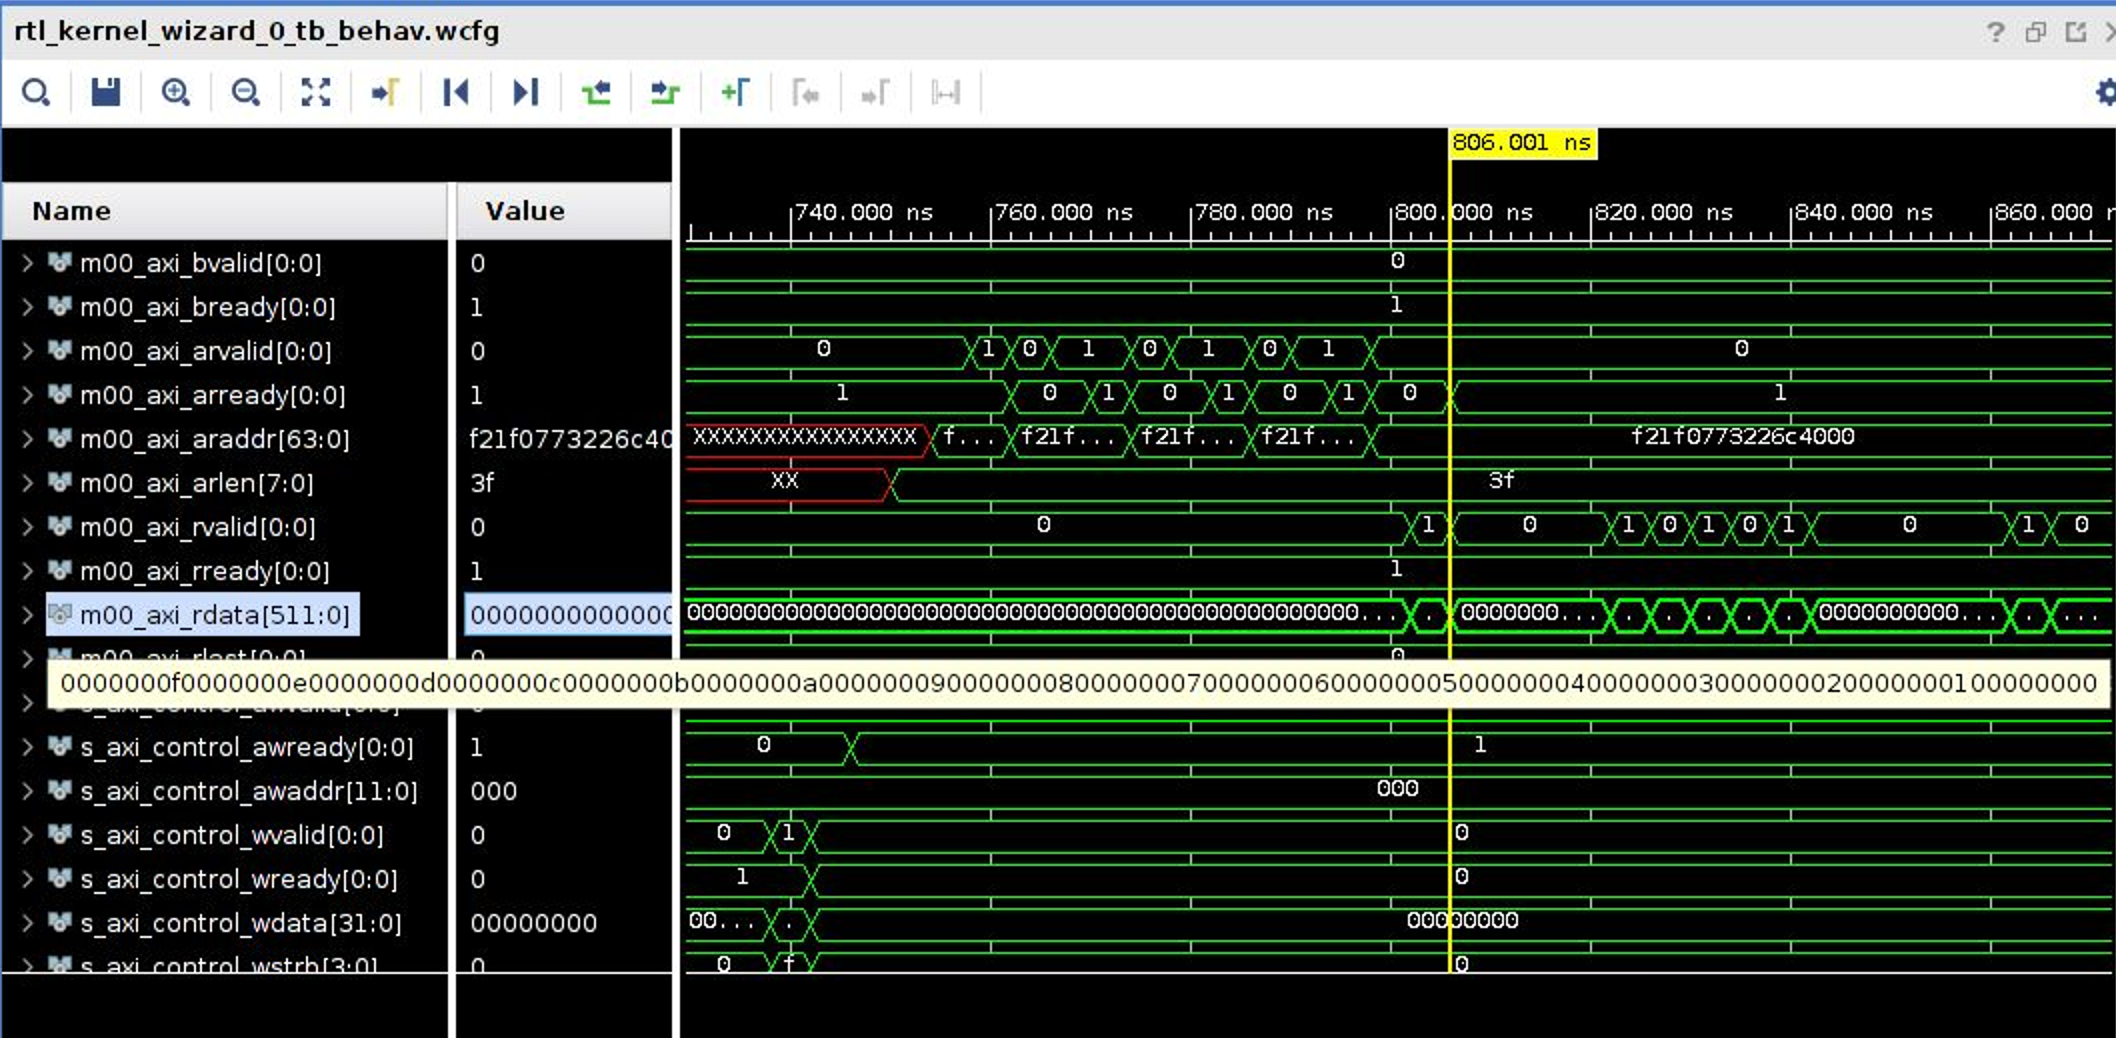
\includegraphics[width = \linewidth]{inc/read.png}
	\caption{Транзакция чтения данных вектора на шине AXI4 MM из DDR памяти}
	\label{readTrans}
\end{figure}
\newpage
Последовательность событий транзакции записи: AWVALID→ AWREADY → WVALID → WREADY → BVALID → BREADY. На рисунке \ref{writeTrans} приведена транзакция записи результата инкремента данных на шине AXI4 MM.

\begin{figure}[h!p]
	\centering
	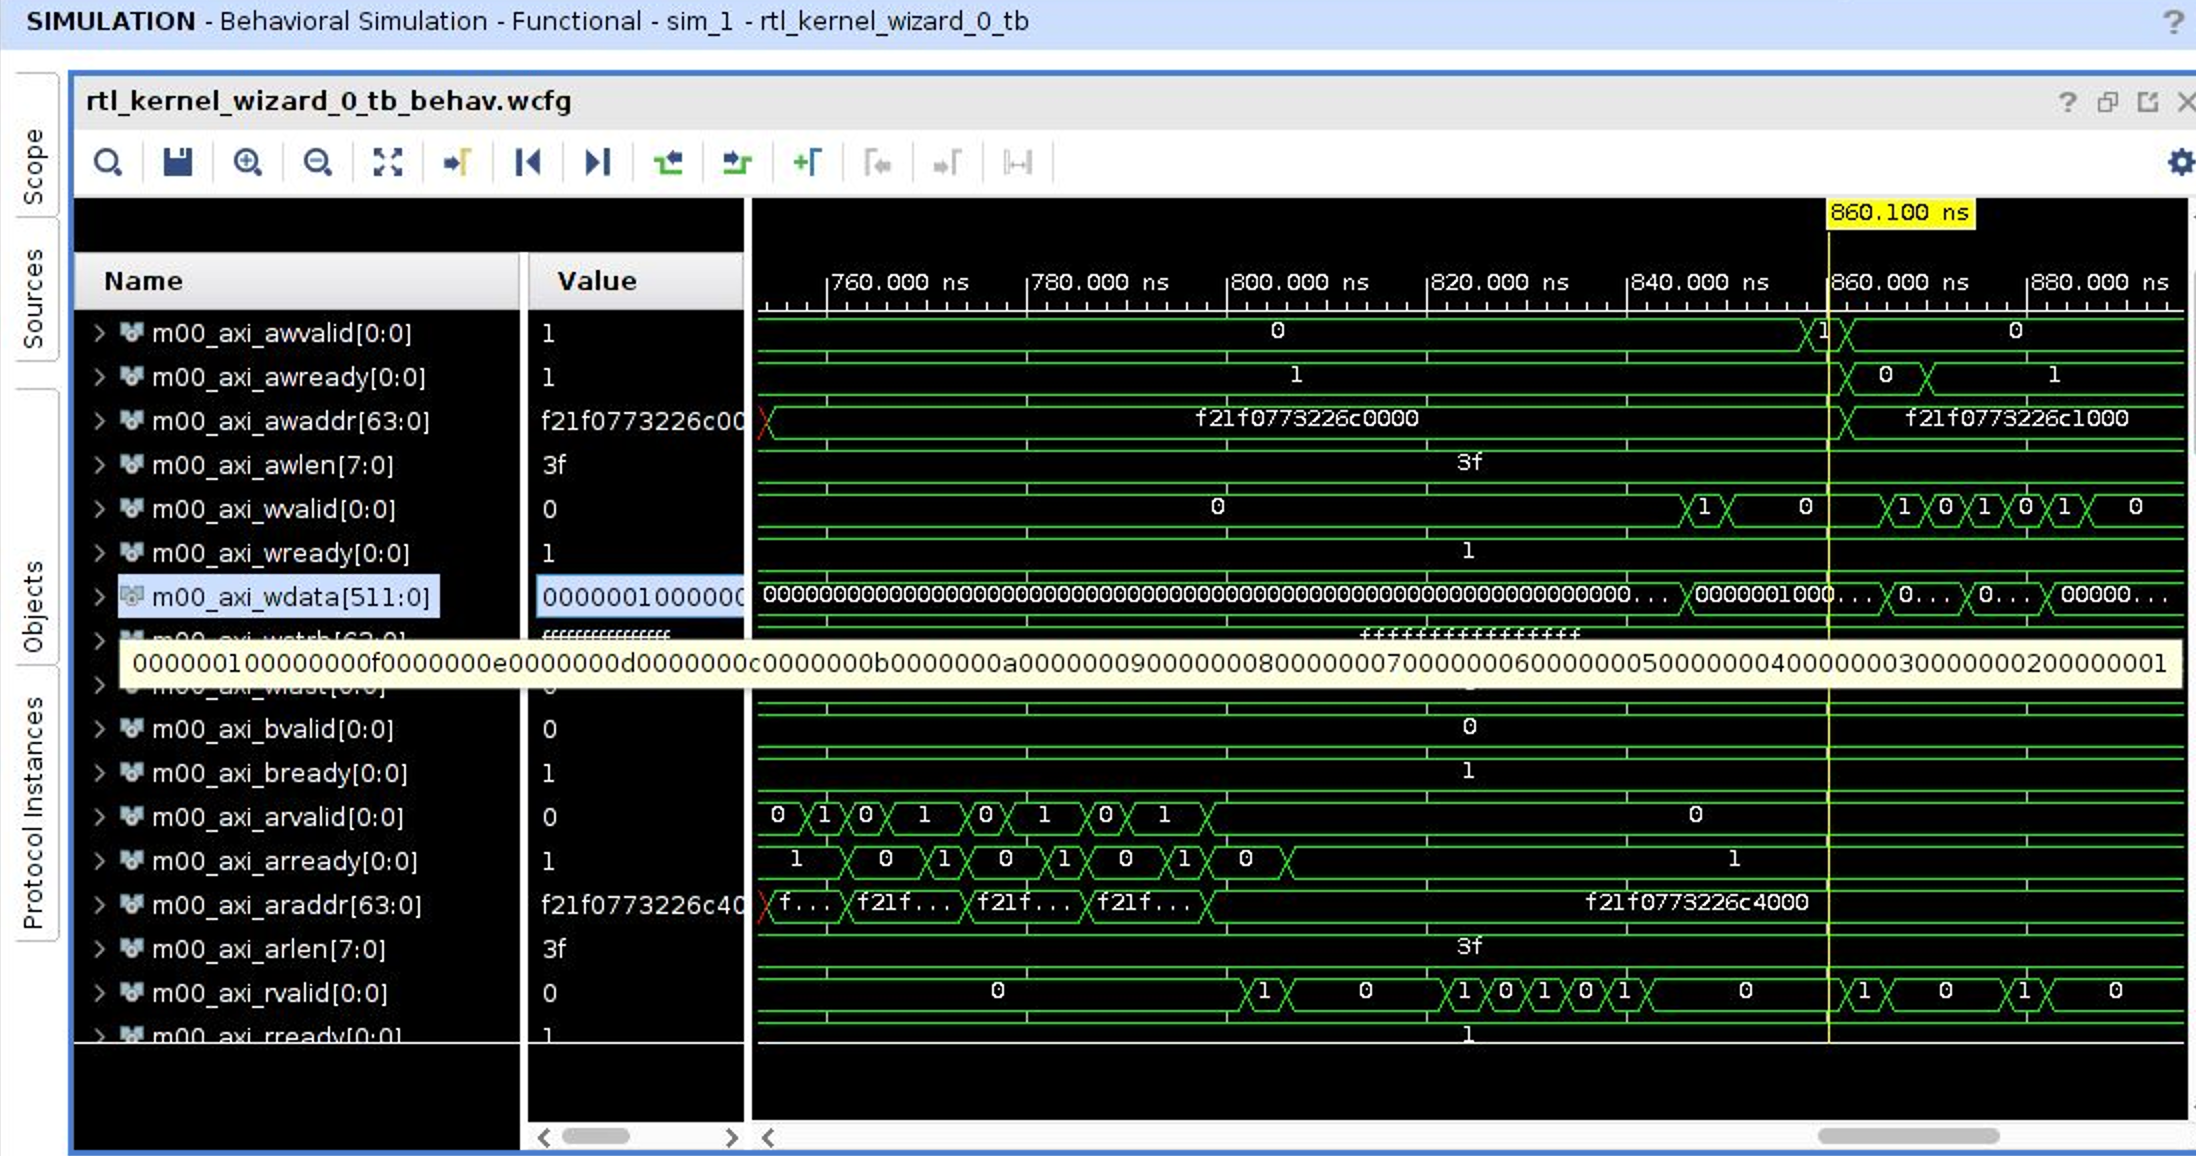
\includegraphics[width = \linewidth]{inc/write.png}
	\caption{Транзакция записи результата инкремента данных на шине AXI4 MM}
	\label{writeTrans}
\end{figure}

На рисунке \ref{incTr} приведен инкремент данных. 

\begin{figure}[h!p]
	\centering
	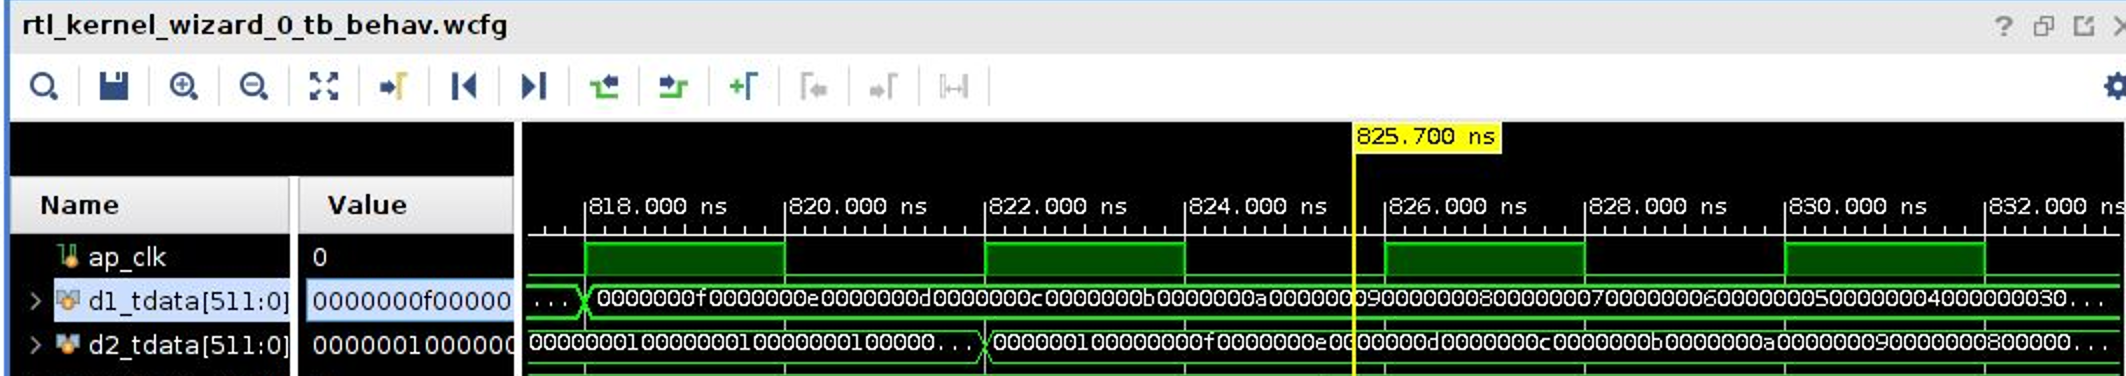
\includegraphics[width = \linewidth]{inc/inc.png}
	\caption{Инкремент данных в модуле}
	\label{incTr}
\end{figure}
\newpage
\section{Симуляция программы индивидуального варианта}
Теперь изменим модуль так, чтобы ускоритель выполнял функцию из индивидуального задания. Сделанные изменения отражены в листинге \ref{func}.
\begin{lstlisting}[label=func,caption=Модифицированная функция]
always @( posedge s_axis_aclk ) begin
    for (i=0; i<LP_NUM_LOOPS; i=i+1) begin
        d2_tdata[i*C_ADDER_BIT_WIDTH+:C_ADDER_BIT_WIDTH] <= (d1_tdata[C_ADDER_BIT_WIDTH*i+:C_ADDER_BIT_WIDTH] > 61680 ? d1_tdata[C_ADDER_BIT_WIDTH*i+:C_ADDER_BIT_WIDTH] : 61680) + 1;
    end
end
\end{lstlisting}

На рисунке \ref{readTransVar} приведена транзакция чтения данных вектора на шине AXI4 MM из DDR памяти.

\begin{figure}[h!p]
	\centering
	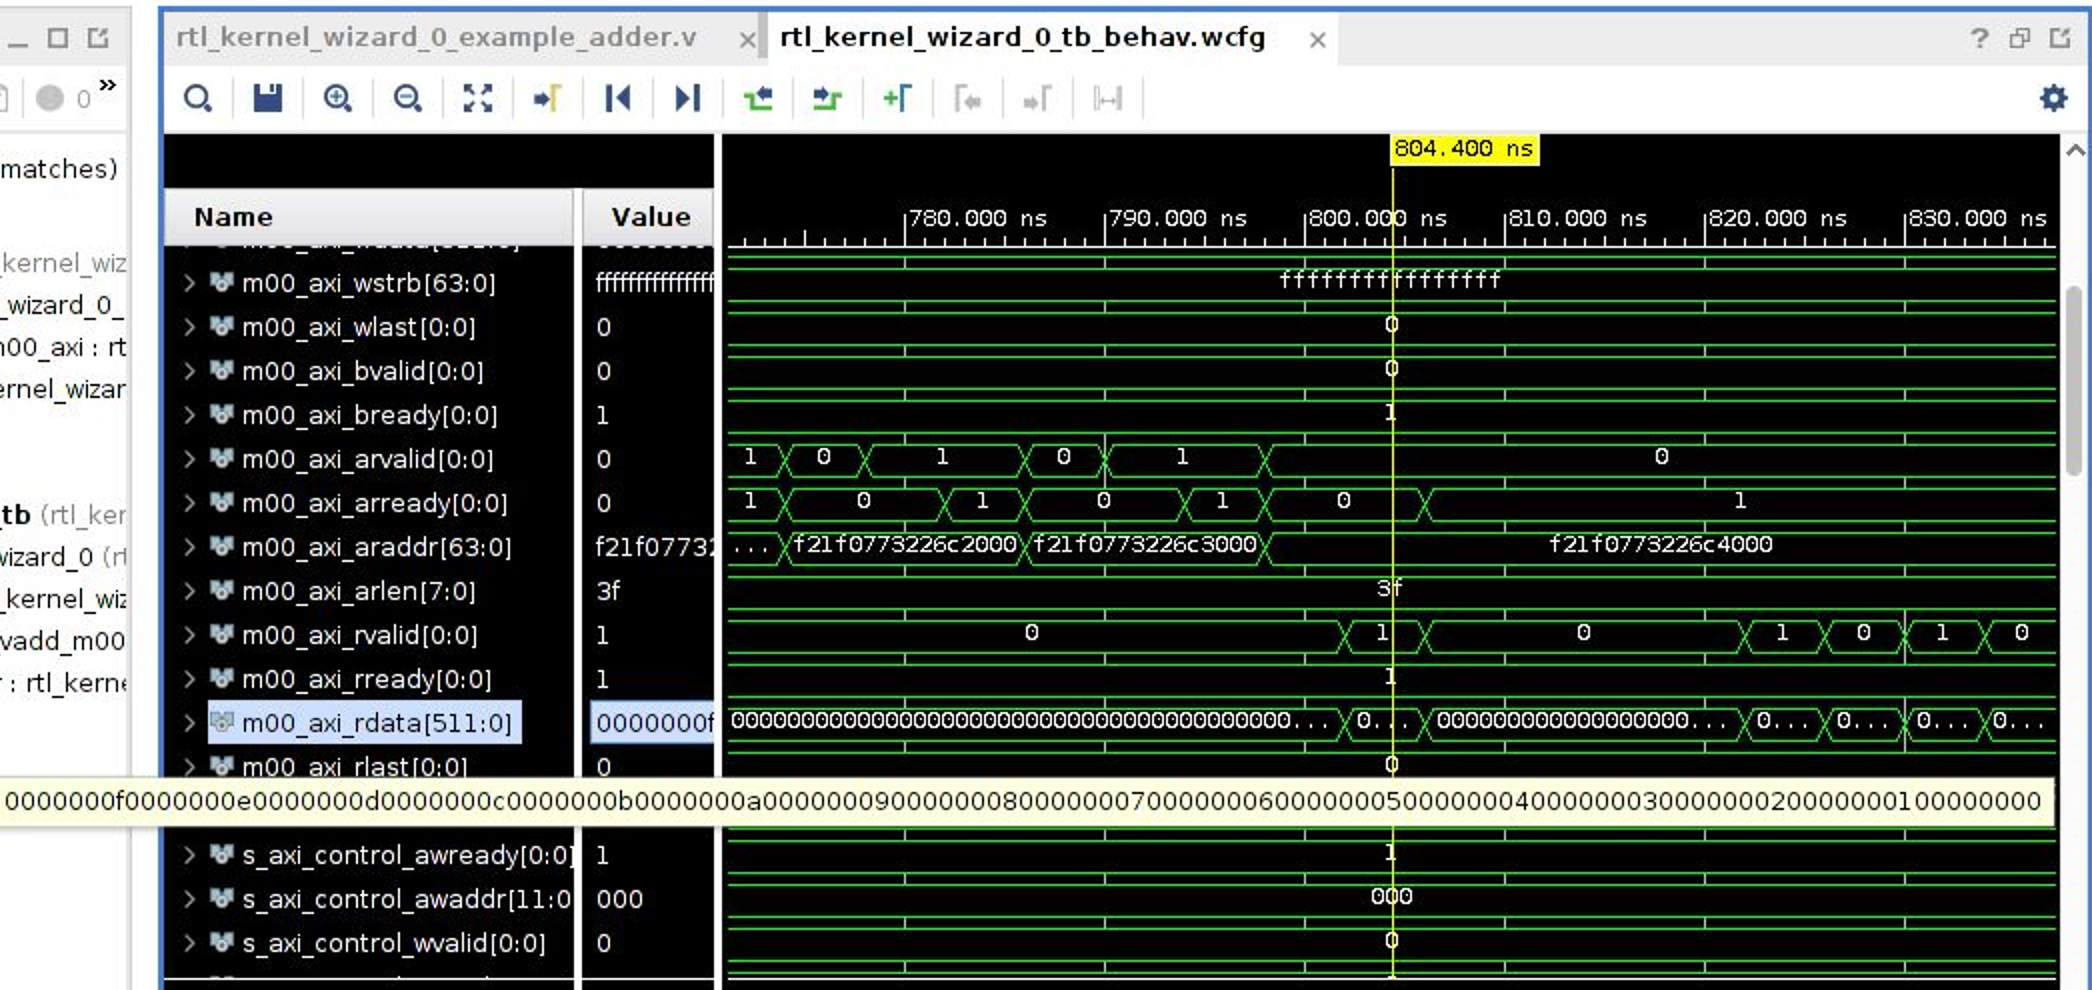
\includegraphics[width = \linewidth]{inc/read_var.png}
	\caption{Транзакция чтения данных вектора на шине AXI4 MM из DDR памяти}
	\label{readTransVar}
\end{figure}
\newpage
На рисунке \ref{writeTransVar} приведена транзакция записи результата инкремента данных на шине AXI4 MM.

\begin{figure}[h!p]
	\centering
	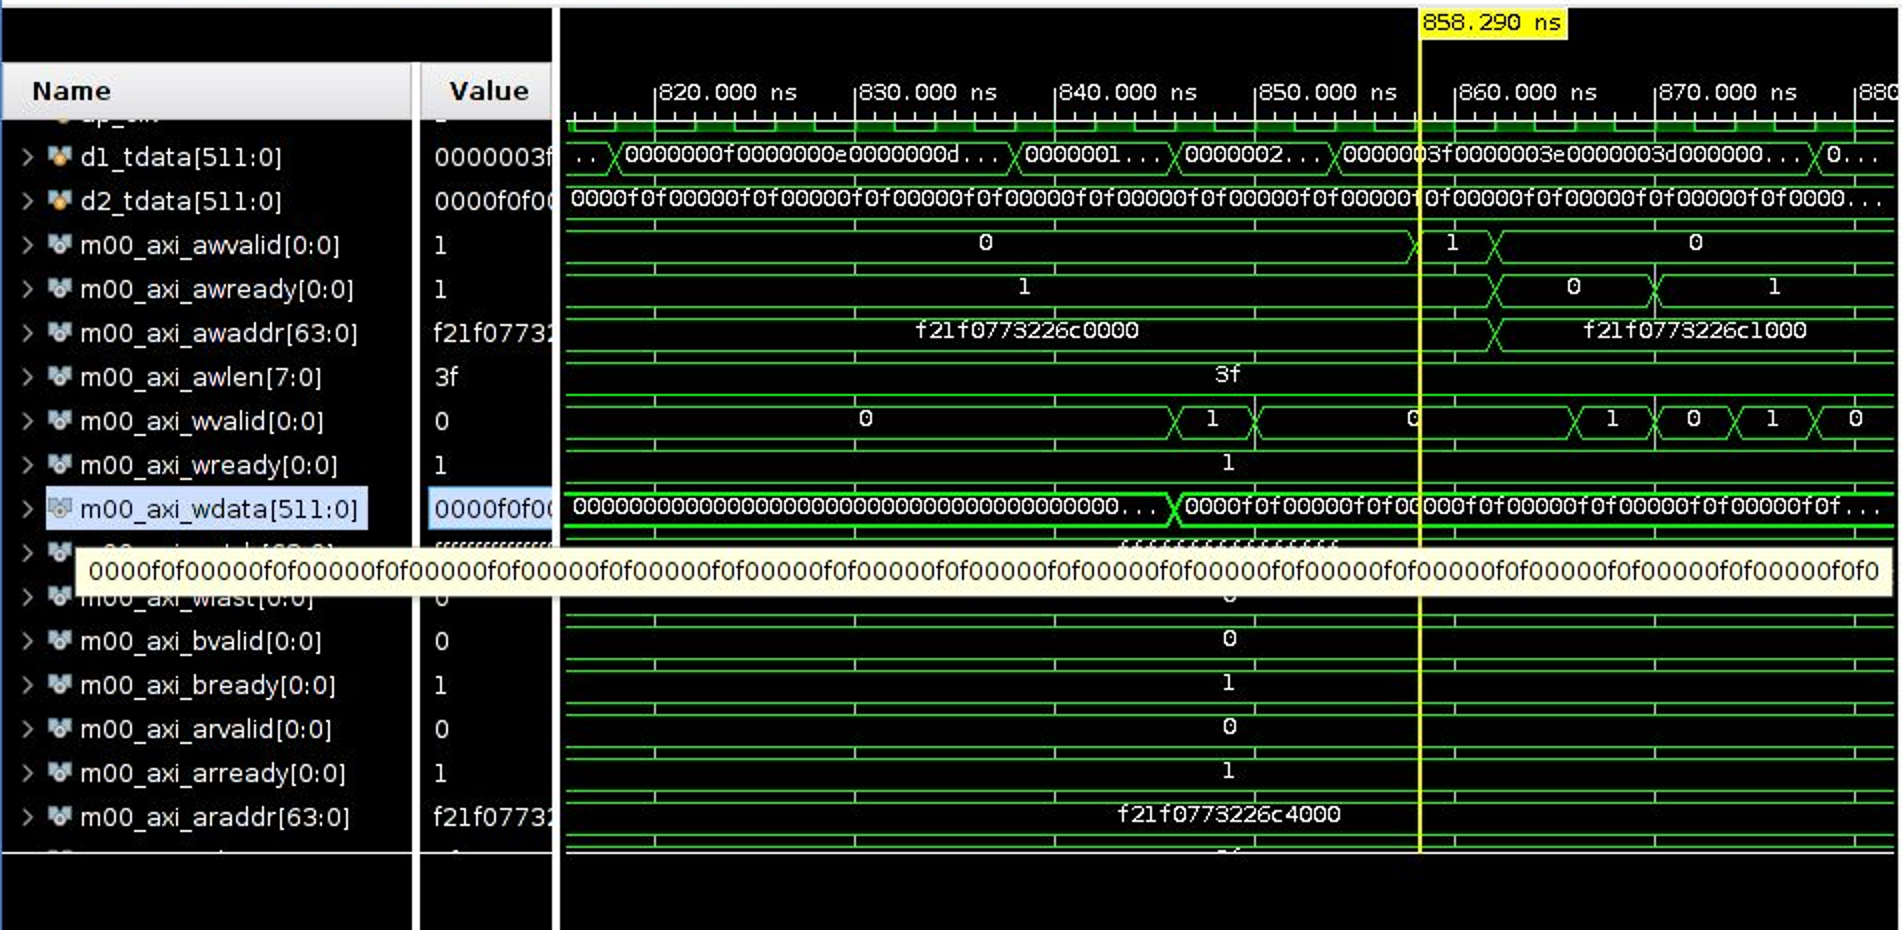
\includegraphics[width = \linewidth]{inc/write_var.png}
	\caption{Транзакция записи результата инкремента данных на шине AXI4 MM}
	\label{writeTransVar}
\end{figure}

На рисунке \ref{incTrVar} приведен инкремент данных. 

\begin{figure}[h!p]
	\centering
	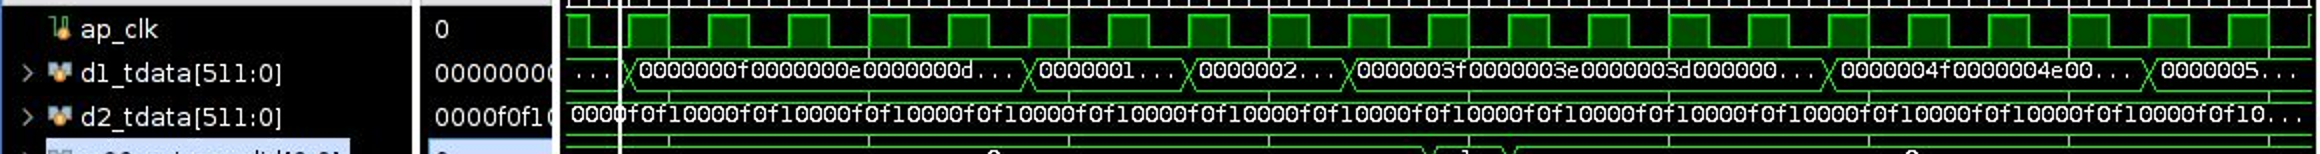
\includegraphics[width = \linewidth]{inc/inc_var.png}
	\caption{Инкремент данных в модуле}
	\label{incTrVar}
\end{figure}

\chapter{Сборка проекта}
В листинге \ref{config} приведено содержимое конфигурационного файла. В соответствии с вариантом требовалось использовать регионы SLR2, DDR[3].
\begin{lstlisting}[label=config,caption=Содержимое файла конфигурации.]
[connectivity]
nk=rtl_kernel_wizard_0:1:vinc0

slr=vinc0:SLR2

sp=vinc0.m00_axi:DDR[3]
sp=vinc0.m00_axi:PLRAM[0]

[vivado]
prop=run.impl_1.STEPS.OPT_DESIGN.ARGS.DIRECTIVE=Explore
prop=run.impl_1.STEPS.PLACE_DESIGN.ARGS.DIRECTIVE=Explore
prop=run.impl_1.STEPS.PHYS_OPT_DESIGN.IS_ENABLED=true
prop=run.impl_1.STEPS.PHYS_OPT_DESIGN.ARGS.DIRECTIVE=AggressiveExplore
prop=run.impl_1.STEPS.ROUTE_DESIGN.ARGS.DIRECTIVE=Explore
\end{lstlisting}

Содержимое файлов v++*.log и *.xclbin.info. приведено в приложениях Б и В.

\chapter{Запуск программного обеспечения на хост-системе}

В листинге \ref{code:hostexample1} приведена измененная части файла host\_example.cpp. Всё содержимое файла приведено в приложении A.

\begin{lstlisting}[label=code:hostexample1, caption=Модуль host\_example.cpp]
// Check Results

for (cl_uint i = 0; i < number_of_words; i++) {
        unsigned res = (h_data[i] > 61680 ? h_data[i] : 61680) + 1;
        if (res != h_axi00_ptr0_output[i]) {
            printf("ERROR in rtl_kernel_wizard_0::m00_axi - array index %d (host addr 0x%03x) - input=%d (0x%x), output=%d (0x%x)\n", i, i*4, h_data[i], h_data[i], h_axi00_ptr0_output[i], h_axi00_ptr0_output[i]);
            check_status = 1;
        }
      //  printf("i=%d, input=%d, output=%d\n", i,  h_axi00_ptr0_input[i], h_axi00_ptr0_output[i]);
    }
\end{lstlisting}

Для отладки и проверки работоспособности была использована утилита xgdb. На рисунке \ref{img:test} приведены результаты тестирования.

\begin{figure}[h!p]
	\centering
	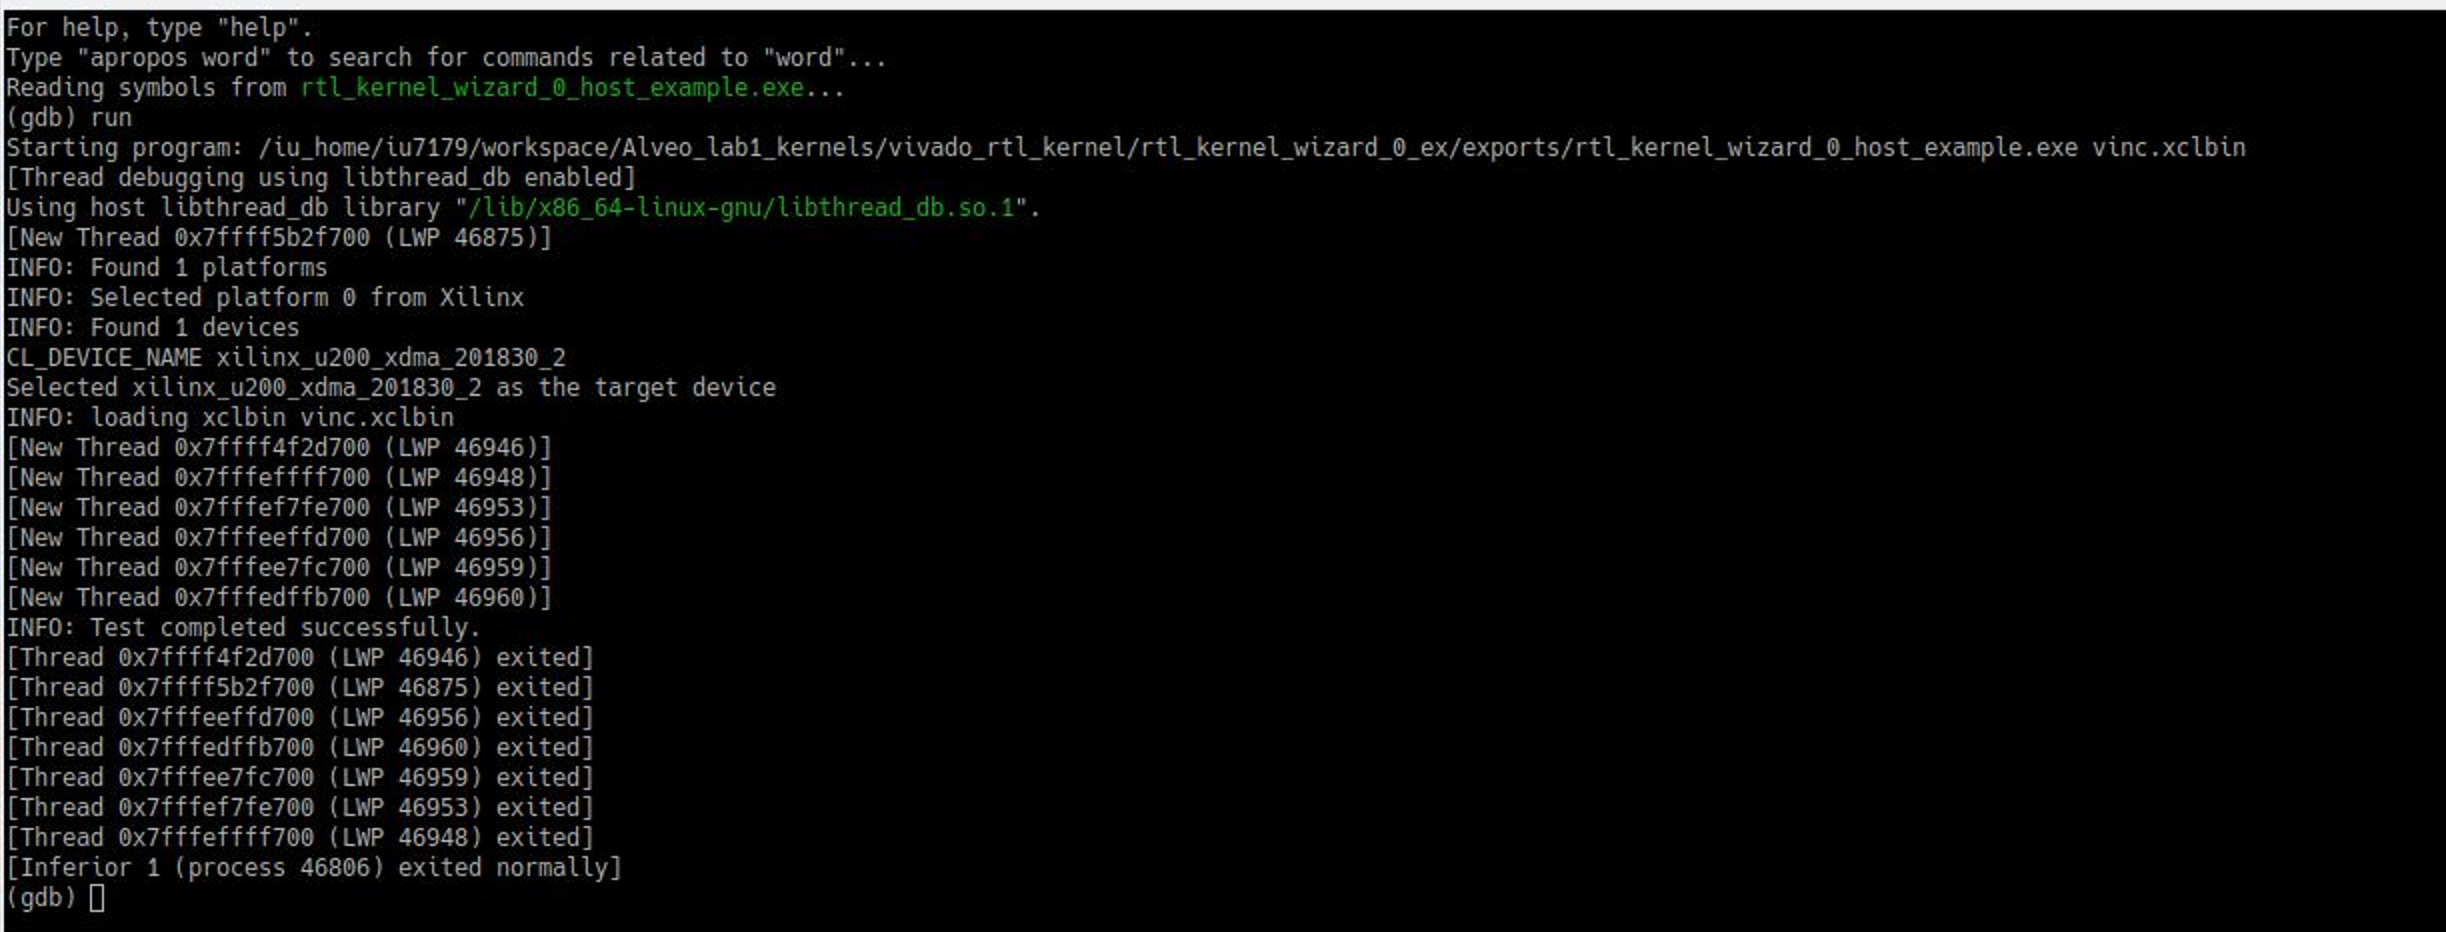
\includegraphics[width = \linewidth]{inc/test.png}
	\caption{Результаты тестирования}
	\label{img:test}
\end{figure}

